\section{Uncertainty design and robustified LP formulation}
\subsection{Uncertainty set design}
\textcolor{red}{Describe here how data were generated. Decision makers have available 5 data points of yearly availability for each item of each seller. 5 years of time-dependent price dynamics were generated (one point every month? State how). For every realization, the price is the same for all the sellers. In contrary, BMP data are not easily available to the plant managers, although some literature values and lab-tests can be performed. Since it is difficult to hypothesized consistently the shape of the BMP distributions, and considering that it represents the most uncertain parameters of the problem, the only assumption that was made is symmetry and existence $\in[-1,1]$ of the perturbations with respect to the deterministic value, in a conservative prospective.}
Da in der Praxis manche Daten besser als andere erhoben bzw. observiert werden können, wurde beim gestalten des uncertainty sets darauf geachtet.
Es  ist praktisch unmöglich die BMP-Kurven jedes Produktes von jedem Verkäufer zu bestimmen. Da dies mit enormen Aufwand und kostenaufwendigen Laboranalysen einhergehen würde.
Daher wurde für die Unsicherheit des BMP einige Annahmen getroffen. Zunächst gehen wir davon aus, dass zwei gleiche Produkte von verschiedenen Verkäufern die selben BMP Kurven haben. Da außerdem in der Praxis keine bzw. sehr wenige Vergangenheitsdaten dafür vorliegen,  nehmen wir an, dass die Verteilung der Abweichungen vom Mittelwert symmetrisch sind. Durch Definition von maximalen Schwankungen kann die Verteilung der Abweichungen auf das Intervall [-1,1] reduziert werden und ein theoretisches Resultat zur Definition des Gamma verwendet werden.
Des Weiteren liegen nur limitierte Daten für der Verfügbarkeit der verschiedenen Produkte vor. Die Produktion eines Produktes und daraus resultierend die Verfügbarkeit am Markt lässt sich relativ gut nachverfolgen. Dagegen ist es fast unmöglich die Verfügbarkeit aller Produkte bei jedem Händler einzeln einzusehen. 
Da wir bei unseren Betrachtungen davon ausgehen, dass alle Verkäufer sehr nahe beieinander produzieren und der Produktionsoutput hauptsächlich aufgrund von exogenen Umweltfaktoren schwankt, kann man davon ausgehen, dass annähernd alle Verkäufer die gleichen Schwankungen haben. Ist zum Beispiel in einem beliebigen Jahr das Wetter sehr ungünstig für die Produktion von Mais, ist davon auszugehen, dass alle Bauern, die auf Freiflächen anbauen gleichermaßen geringere Mengen Mais produzieren. Daher wird für die Berechnung eines Gammas für die Kapazitätsgrenzen nur ein Wert pro Jahr generiert. Für die Generierung des zufälligen Angebots sind aus historischen Daten Minima, Maxima und Durchschnitte gegeben. Daraus und mithilfe einer Beta-Verteilung werden dann konkrete Realisationen der Verfügbarkeiten über die letzten 5 Jahre bestimmt. Es wird davon ausgegangen, dass die Produzenten entsprechend ihrer vordefinierten Größe anteilg die Restmengen zur Verfügung stellen.
Gegenteilig sind Preise für einzelne Produkte einfach nachzuverfolgen und sollten in der Praxis vorliegen. Da die Preise durch den Markt standardisiert sind, haben alle Produkte aller Produzenten an einem gewissen Zeitpunkt immer den gleichen Preis. Die Marktpreise aktualisieren sich wöchentlich. Da uns hier auch nur Minimum, Maximum und Mittelwert der Preise vorliegen, wurde erneut auf die Beta-Verteilung zur Simulation von Daten zurückgegriffen. An dieser Stelle gehen wir noch nicht auf saisonale Schwankungen der Preise ein, dies wäre jedoch eine sinnvolle Anpassung unserer Arbeit. Indem der Planungshorizont auf Quartale reduziert wird, könnte man das Gamma für die Preise auf Basis von saisonalen Daten bestimmen und so deutlich weniger konservative Lösungen erhalten. Da zunächst nur auf einen ganzjährige Plaungshorizont eingegangen wird, wurden die Daten folgendermaßen generiert:
Wir gehen davon aus, dass über ein Jahr die Preise um einen gewissen Wert schwanken. Dieser Wert wurde durch die oben genannte Beta-Verteilung bestimmt. Darüber hinaus werden in den 51 Folgewochen zufällige Inkremente gezogen. Da weder Trend noch saisonale Schwankungen existieren sollen, werden die Inkremente symmetrisch mittels einer Dreiecksverteilung zwischen -0,5 und +0,5 zufällig bestimmt. Das Folgejahr erhält einen neuen Wert aus der Beta Verteilung und darauffolgend wieder 51 symmetrisch Verteilte Inkremente, usw.
Dabei sollen die Inkremente die oberen bzw. unteren Schranken der Preise, welche für jedes Produkt unterschiedlich sind, nichtverletzen. Und werden daher an den Schranken abgeschnitten. Insgesamt ergeben sich 5×52 Datenpunkte für jedes Produkt. Offensichtlich sind die Preiskurven nicht realistisch, da es besonders zu Jahreswechsel zu großen Sprüngen kommen kann. Da jedoch für Robuste Optimierung eine Worst Case Analyse durchgeführt wird, beeinträchtigen diese Sprünge in den Preiskurven nicht die Güte der Lösung. Da in der Praxis die echten Preiskurven jedes Produktes vorliegen sollten, kann bei der Anwendung einfach die zufällige Datengenerierung durch die gespeicherten Preiskurven ersetzt werden und somit realistische Gamma errechnet werden.

\begin{figure*}[htb]
 \begin{center}
  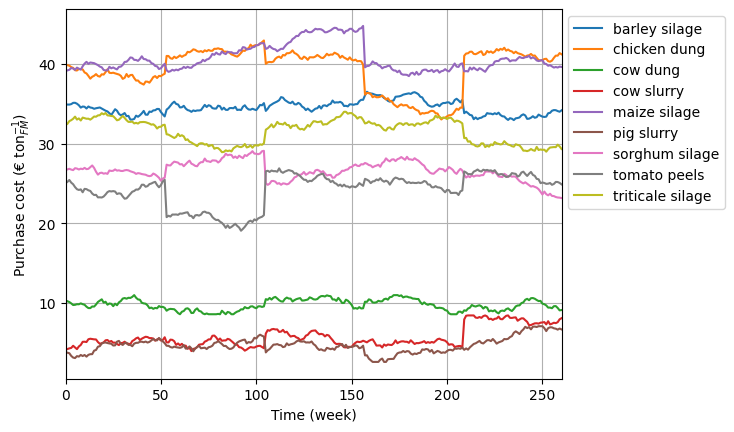
\includegraphics[width=1\columnwidth]{./img/Pricedata_2024-05-07.png}
 \end{center}
 \caption{Generated price data time series for each item}
 \label{fig:dataprice}
\end{figure*}

For a first design of uncertainty, all sources were included in the problem formulation separately, so that 3 different random variables were introduced. Since price and BMP$_\infty$ are very unlikely to be correlated, designing uncertainty separately could be overly conservative (i.e. both taking extreme values for the same realization), but it was reasoanable for first attempts and for being able to assess the sensitivity of J to each of them too. On the other hand, price realizations are likely to have a correlation with item availabilities.
Table \ref{tab:randomvar} reports the same nomenclature that is found in the COLAB to discriminate between the different sources of uncertainty. The uncertainty sets (formalized in Eq.\ref{eq:sets}) were all designed as budgeted sets to avoid being too conservative (es. with box sets). Budgeted was choose over ellipsoidal sets just to preserve the linearity (over convexity) of the robust counterpart. 
The sets are similarly formalized as below for random variable, i.e.:
\begin{equation}\label{eq:sets}
\begin{aligned}
    \mathcal{Z}:=\{z\in\mathbb{R}^n\,|\,z\in[-1,\,1]^n,\|z\|_1 \leq \Gamma_Z\}\,\\
    \mathcal{W}:=\{w\in\mathbb{R}^n\,|\,w\in[-1,\,1]^n,\|w\|_1 \leq \Gamma_W\}\,\\
    \mathcal{L}:=\{l\in\mathbb{R}^n\,|\,l\in[-1,\,1]^n,\|l\|_1 \leq \Gamma_L\}\,
\end{aligned}
\end{equation}
% Table generated by Excel2LaTeX from sheet 'For Report'
\begin{table*}[htbp]
  \centering
  \caption{Nomenclature as present in COLAB for the different uncertanity sources}
    \begin{tabular}{SlScScSc}
    \toprule
    Source of uncertainty & Random variable & Uncertanty Set & Set size parameter \\
    \midrule
    Availability & z     & availabilitySet     & Gamma\_availability \\
    Prices & w     & pricesSet     & Gamma\_price \\
    BMPinf & l     & BMPSet     & Gamma\_BMP \\
    \bottomrule
    \end{tabular}%
  \label{tab:randomvar}%
\end{table*}%
The size parameter was firstly calibrated in order for $\mathcal{Z,W}$ and $\mathcal{L}$ to be such that a robust linear constraint employing $z,w$ or $l$ is guaranteed to satisfy the chance constraint with Prob\% (95\%) probability (Theorem 3.2 of lecture notes).

As shown in Fig.\ref{fig:distribdata}, the generated price data were not symmetric, so that Theorem 3.5 of the lecture notes could not apply. For this reason, it was chosen to design the size parameters based on the actual distribution of data.

\begin{figure*}[htb]
 \begin{center}
  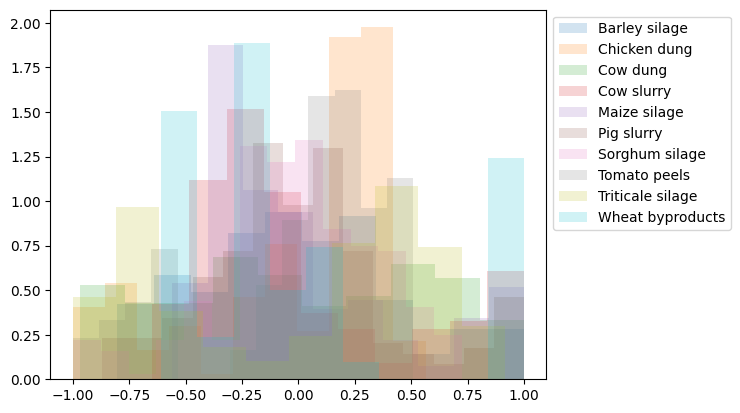
\includegraphics[width=1\columnwidth]{./img/Distribution_price_2024-05-06.png}
 \end{center}
 \caption{Histograms of $Z_P$ for each item}
 \label{fig:distribdata}
\end{figure*}

Data were first standardized as for Eq.\ref{eq:standardize} to be consistent with the definition of random variables as "perturbation" with respect to the mean values, i.e.:
\begin{equation}\label{eq:standardize}
\begin{aligned}
    R_A = \mu_A +P_A Z_A, \\
    R_P = \mu_P +P_P Z_P
\end{aligned}
\end{equation}
where $\mu$ contains the mean realizations, $P\in \mathbb{R}^{n \times n}$ are diagonal matrices containing the maximum deviations, $Z_A \in \mathbb{R}^{n \times 5}$ and $Z_P \in \mathbb{R}^{n \times 260}$ are the matrices that contain all the standardized realization of availabilities and prices respectively.
The latter were thus sorted based on their norm-one; the value that corresponded to the desired P was considered as $\Gamma_Z$ and $\Gamma_W$. 
It is noteworthy to highlight that, due to the very few realizations of availability, the design of $\Gamma_Z$ was very much impacted by rounding in quantizing the sorted realizations.

The size of the uncertainty set for BMP$_\intfty$ was computed as suggested by Theorem 3.5:
\begin{equation*}
   \Gamma_L = \sqrt{2 n \log_{10} \frac{1}{1-P}} 
\end{equation*}
%------------------------------------------------------------------
\subsection{R-LP formulation}
Because of two sources of uncertainty being present in the formulation of \emph{J}, the latter was re-written in forms of two inequality constraints on revenues and operational expenditures.
The robustifed problem ('R-LP') was thus formulated as:
\begin{eqnarray*}
\max_{x\in\chi,s,c}&&J=s-c\\
\mbox{s.t.} && s \leq \sum_{i=1}^{n}\sum_{j=1}^{m} p_{ch4} BMP_{i} VS_{i} \frac{x_{i,j}}{N} \forall l=1,\dots,L\\
&& c \geq \sum_{i=1}^{n}\sum_{j=1}^{m} (C_{Pi,j} +C_{Ti,j})\frac{x_{i,j}}{N}\forall z=1,\dots,Z\\
&& \frac{\sum_{j=1}^{m}\sum_{i=1}^{n\in R} x_{i,j}}{\sum_{j=1}^{m}\sum_{i=1}^{n} x_{i,j}} \lessgtr RL_{r} \ \forall r=1,\dots,R\\
&& x_{i,j} \leq A_{i,j} \ \forall i=1,..,n,\ \forall j=1,..,m,\ \forall w=1,..,W\\
&& k_{min}\leq \frac{\sum_{i=1}^{n}\sum_{j=1}^{m} k_i x_{i,j}}{\sum_{i=1}^{n}\sum_{j=1}^{m} x_{i,j}}\leq k_{max}\ \forall k=1,\dots,K\,\\
&& \frac{\sum_{i=1}^{n}\sum_{j=1}^{m} (BMP_{\infty,i}-BMP_{i}) x_{i,j}}{\sum_{i=1}^{n}\sum_{j=1}^{m} BMP_{i} x_{i,j}}\leq BMP_{res,max}\\\
&& HRT = \frac{V_RN}{\sum_{i=1}^{n}\sum_{j=1}^{m} x_{i,j}}\\
&& x_{i,M} = A_{i,M}\ \forall i=1,\dots,n\\
&& x_{i,j}\geq 0\ \forall i=1,\dots,n\ \forall j=1,\dots,m\\
\end{eqnarray*}

In the formulation above, the following equalities hold:
\begin{eqnarray*}
BMP(HRT,l) = && \overline{BMP(HRT)}\left(1+\left(1-\frac{BMP_{\infty,min}}{\overline{BMP_{\infty}}}\right)l\right ),\\
BMP_{\infty}(l) = && \overline{BMP_\infty}\left(1+\left(1-\frac{BMP_{\infty,min}}{\overline{BMP_{\infty}}}\right)l\right ),\\
C_P(w) = && bm(\mu_{P} +P_{P} w),\\
A(z) = && (ss^T(\mu_A +P_A z))^T
\end{eqnarray*}
where $bm$ is the binary matrix than indicates the presence of the items at the sellers, $ss$ is a matrix that indicates the re-partition of the overall items availability as proportional to the different seller "sizes" and $\overline{BMP(HRT)}, \overline{BMP_{\infty}}$ are the deterministic values of the conversion yield at the given HRT and the maximum achievable, respectively.

The hard constraint that forces the consumption of what is produced by the plant itself (\emph{j=M}) could not be easily robustified, so that it was left as in the deterministic form (the plant manager is fairly more confident on its own plant future production).